\pdfminorversion=4
\documentclass[aspectratio=169]{beamer}

\mode<presentation>
{
  \usetheme{default}
  \usecolortheme{default}
  \usefonttheme{default}
  \setbeamertemplate{navigation symbols}{}
  \setbeamertemplate{caption}[numbered]
  \setbeamertemplate{footline}[frame number]  % or "page number"
  \setbeamercolor{frametitle}{fg=white}
  \setbeamercolor{footline}{fg=black}
} 

\usepackage[english]{babel}
\usepackage[utf8x]{inputenc}
\usepackage{tikz}
\usepackage{courier}
\usepackage{array}
\usepackage{bold-extra}
\usepackage{minted}
\usepackage[thicklines]{cancel}
\usepackage{fancyvrb}

\xdefinecolor{dianablue}{rgb}{0.18,0.24,0.31}
\xdefinecolor{darkblue}{rgb}{0.1,0.1,0.7}
\xdefinecolor{darkgreen}{rgb}{0,0.5,0}
\xdefinecolor{darkgrey}{rgb}{0.35,0.35,0.35}
\xdefinecolor{darkorange}{rgb}{0.8,0.5,0}
\xdefinecolor{darkred}{rgb}{0.7,0,0}
\definecolor{darkgreen}{rgb}{0,0.6,0}
\definecolor{mauve}{rgb}{0.58,0,0.82}

\title[2019-04-24-irishep-skyhook]{Skyhook for query systems}
\author{Jim Pivarski}
\institute{Princeton University -- IRIS-HEP}
\date{April 24, 2019}

\usetikzlibrary{shapes.callouts}

\begin{document}

\logo{\pgfputat{\pgfxy(0.11, 7.4)}{\pgfbox[right,base]{\tikz{\filldraw[fill=dianablue, draw=none] (0 cm, 0 cm) rectangle (50 cm, 1 cm);}\mbox{\hspace{-8 cm}
\includegraphics[height=1 cm]{princeton-logo-long.png}\hspace{0.1 cm}\raisebox{0.1 cm}{
\includegraphics[height=0.8 cm]{iris-hep-logo-long.png}}\hspace{0.1 cm}}}}}

\begin{frame}
  \titlepage
\end{frame}

\logo{\pgfputat{\pgfxy(0.11, 7.4)}{\pgfbox[right,base]{\tikz{\filldraw[fill=dianablue, draw=none] (0 cm, 0 cm) rectangle (50 cm, 1 cm);}\mbox{\hspace{-8 cm}
\includegraphics[height=1 cm]{princeton-logo.png}\hspace{0.1 cm}\raisebox{0.1 cm}{
\includegraphics[height=0.8 cm]{iris-hep-logo.png}}\hspace{0.1 cm}}}}}

% Uncomment these lines for an automatically generated outline.
%\begin{frame}{Outline}
%  \tableofcontents
%\end{frame}

% START START START START START START START START START START START START START

\begin{frame}{My view of the world}
\vspace{0.25 cm}
\begin{center}
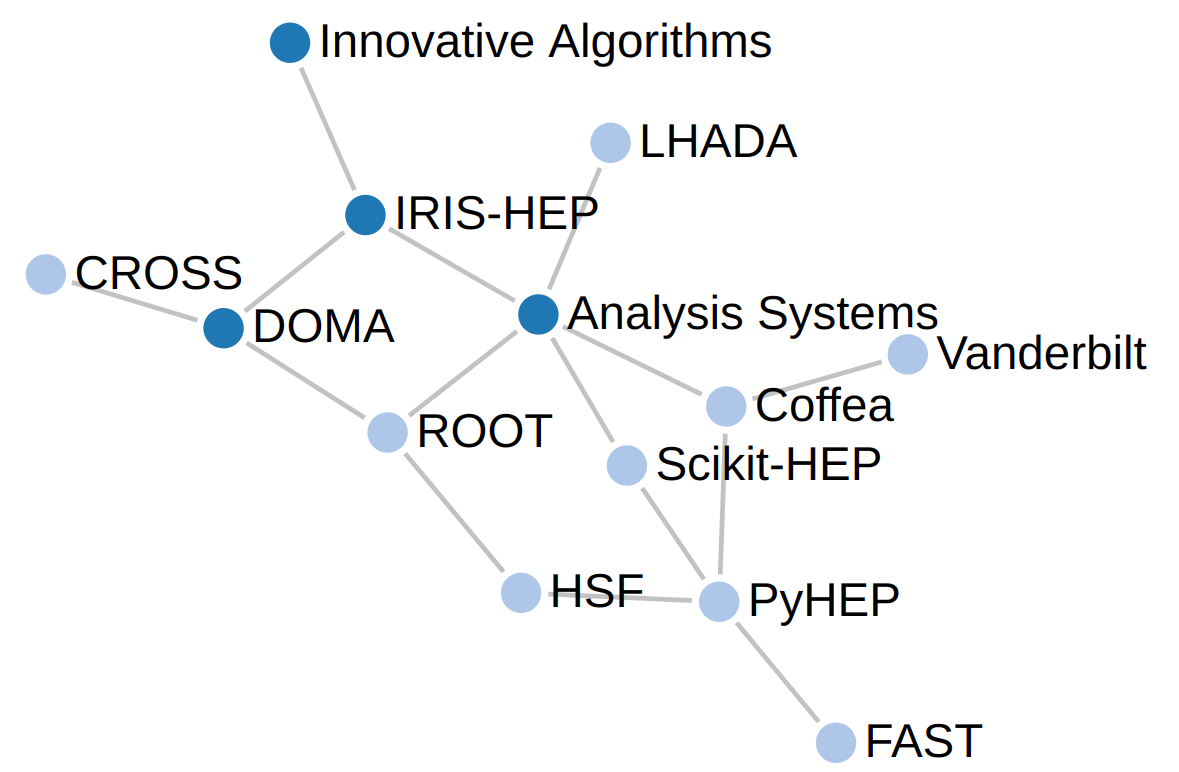
\includegraphics[width=0.8\linewidth]{analysis-connections-cross.png}
\end{center}

\scriptsize
\vspace{-2.5\baselineskip}
Biased? Incomplete? Help me fix it.

\textcolor{blue}{\url{https://github.com/iris-hep/analysis-connections}}
\end{frame}

\begin{frame}{Building an ntupleless future}
\vspace{0.5 cm}
\Large {\bf Query System:} big data on server, users request reduced output
\begin{center}
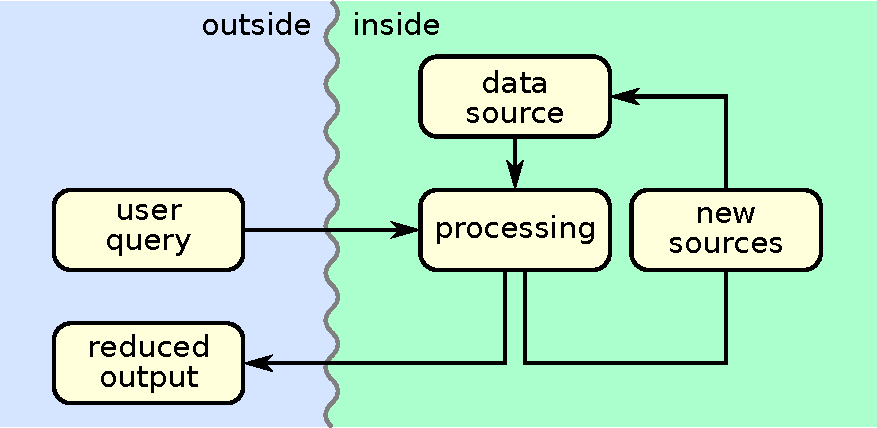
\includegraphics[width=0.6\linewidth]{basic-block-diagram.pdf}
\end{center}

\normalsize
\begin{itemize}
\item \textcolor{darkblue}{Mark Neubauer, Ben Galewsky:} query scheduling, data delivery, iDDS
\item \textcolor{darkblue}{Gordon Watts, Emma Torro, Mason Proffitt:} query expression language
\item \textcolor{darkblue}{Jim Pivarski, Henry Schreiner:} event data processing, histogram aggregation
\end{itemize}
\end{frame}

\begin{frame}{Working closely with analysis groups}
\vspace{0.75 cm}
\begin{columns}
\column{0.2\linewidth}

\includegraphics[width=\linewidth]{coffea-logo.png}

\column{0.8\linewidth}
\hspace{-0.2 cm}\Huge Coffea

\vspace{0.25 cm}
\large {\bf C}olumnar {\bf O}bject {\bf F}ramework {\bf F}or {\bf E}ffective {\bf A}nalysis

\vspace{0.25 cm}
\normalsize Matteo~Cremonesi, Lindsey~Gray, Oliver~Gutsche, Allison~Hall, Bo~Jayatilaka, Igor~Mandrichenko, Kevin~Pedro, Nick~Smith~[FNAL]
\end{columns}

\vspace{0.25 cm}
\begin{center}
\begin{minipage}{0.85\linewidth}
\large Performing two complete CMS analyses
\begin{itemize}
\item Dark Higgs search
\item Boosted SM $H \to b\bar{b}$
\end{itemize}
using my \textcolor{darkblue}{awkward-array event processing}, Ben's \textcolor{darkblue}{distributed processing with Spark}, and Andrew Melo's \textcolor{darkblue}{Spark cluster at Vanderbilt}.
\end{minipage}
\end{center}
\end{frame}

\begin{frame}{Data granularity}
\large
\vspace{0.5 cm}
We've found that it's useful to work with analysis data as individual ROOT branches converted into jagged arrays, rather than event records.
\begin{itemize}
\item efficient processing in Python
\item analysis code readability
\item \textcolor{darkblue}{columnar granularity}
\end{itemize}

\vspace{0.5 cm}
\uncover<2->{One-plot queries (not yet realistic) would require $<1$\% of the columns but nearly all of the rows (events).}

\vspace{0.5 cm}
\uncover<2->{Whole-analysis workflows (demonstrated with Coffea) require $\sim 10$\% of the columns with loose trigger cuts.}

\vspace{0.5 cm}
\uncover<3->{\textcolor{darkblue}{For applications like this, the unit of data is columns, not files or events.}}
\end{frame}

\begin{frame}{Data delivery to query system}
\large
\vspace{0.5 cm}
One of IRIS-HEP DOMA's projects is to create an \textcolor{darkblue}{intelligent Data Delivery System (iDDS)}, which would respond to requests for data in high-level terms (\textcolor{gray}{``muon kinematics in the first million events of 2018 data''}), rather than low-level terms (\textcolor{gray}{``bytes 1024--2048 of some/file.root''}).

\vspace{0.5 cm}
\uncover<2->{For query applications, we would be requesting column segments, maybe with very simple cuts (e.g.\ trigger lines). Complex filtering happens in query system.}

\vspace{0.5 cm}
\begin{uncoverenv}<3->
This is a good match to what Skyhook can deliver:
\begin{itemize}
\item format-aware data delivery;
\item reformatting: decompression, recompression, concatenation, slicing;
\item intelligence close to the source.
\end{itemize}
\end{uncoverenv}
\end{frame}

\begin{frame}{The ROOT file format is complicated}
\large
\vspace{0.5 cm}
Just finding the bytes for \textcolor{gray}{``muon $p_T$ in events 1--1000''} is a non-trivial task, requiring infrastructure like ROOT, uproot, groot, root4j, etc.---which places limits on how ``close to storage'' the intelligence can go.

\vspace{0.5 cm}
\uncover<2->{However, each logical entity {\it has} a fixed byte range in the files. A full framework can identify these ranges and a save them to an index to simplify lookups.}

\vspace{0.5 cm}
\uncover<3->{\textcolor{blue}{\small\url{https://github.com/diana-hep/uproot-skyhook}} uses uproot to map logical row/entry numbers and column names to TBasket locations in the ROOT files. The index is formatted as Flatbuffers (Jeff's preferred format)---any process that can read Flatbuffers can deliver jagged arrays from the indexed ROOT files.}
\end{frame}

\begin{frame}[fragile]{Sample: the Flatbuffers schema}
\scriptsize
\begin{columns}[t]
\column{0.5\linewidth}
\begin{minted}{protobuf}
include "interpretation.fbs";

enum Compression: int {
  none = 0,
  zlib = 1,
  lzma = 2,
  old = 3,
  lz4 = 4
}

table Branch {
  local_offsets: [ulong] (required);
  page_seeks: [ulong] (required);
  compression: Compression;
  iscompressed: [bool];
  compressedbytes: [uint];
  uncompressedbytes: [uint] (required);
  basket_page_offsets: [uint] (required);
  basket_keylens: [uint];
  basket_data_borders: [uint];
}
\end{minted}

\column{0.5\linewidth}
\begin{minted}{protobuf}
table Column {
  interp: uproot_skyhook
      .interpretation_generated
      .Interpretation (required);
  title: string;
}

table File {
  location: string (required);
  uuid: string (required);
  branches: [Branch] (required);
}

table Dataset {
  name: string (required);
  treepath: string (required);
  colnames: [string] (required);
  columns: [Column] (required);
  files: [File] (required);
  global_offsets: [ulong] (required);
  location_prefix: string;
}
\end{minted}

\end{columns}
\end{frame}

\begin{frame}{Current status---before seeing Jeff's talk today!}
\Large
\vspace{0.5 cm}
\begin{itemize}\setlength{\itemsep}{0.5 cm}
\item What Skyhook provides is a good match to what iDDS is trying to achieve.
\item The unit of data for a query system is a column segment.
\item I provided Jeff with a way to generate mappings from high-level entities---row/entry numbers and column names---to low-level byte positions.
\item Once a prototype works, it could be tested with Coffea.
\end{itemize}
\end{frame}

%% \begin{frame}{Data formats, delivery mechanisms}
%% \large
%% \vspace{0.5 cm}
%% For various reasons, Coffea analyses have used \textcolor{darkblue}{ROOT files} (most direct), \textcolor{darkblue}{CouchBase} (Striped data delivery service), \textcolor{darkblue}{Parquet files} (Spark), and \textcolor{darkblue}{ZIP files of arrays} (Numpy native).

%% \vspace{0.5 cm}
%% They all deliver jagged arrays.

%% \vspace{0.5 cm}
%% \uncover<2->{Ideally, the query service should get data from a component that}

%% \vspace{0.1 cm}
%% \begin{itemize}
%% \item<2-> understands the format well enough to deliver logical arrays, not raw bytes;
%% \item<3-> doesn't double disk space with a secondary format;
%% \item<4-> puts intelligence close to the source to avoid unnecessary transfers.
%% \end{itemize}

%% \vspace{0.25 cm}
%% \uncover<5->{In IRIS-HEP Analysis Systems, we're calling such a service iDDS.}
%% \end{frame}

%% \begin{frame}{Which is why Skyhook can help}
%% \large
%% \vspace{0.5 cm}
%% The goals align well with iDDS, demonstrated with a successful application.

%% \vspace{0.5 cm}
%% \begin{columns}
%% \column{0.47\linewidth}
%% \underline{PostgreSQL Application}

%% \begin{itemize}
%% \item delivers SQL tables
%% \end{itemize}

%% \column{0.47\linewidth}
%% \underline{ROOT Application}

%% \begin{itemize}
%% \item delivers jagged arrays


%% \end{itemize}
%% \end{columns}
%% \end{frame}


\end{document}
